\documentclass[]{article}
\usepackage{lmodern}
\usepackage{amssymb,amsmath}
\usepackage{ifxetex,ifluatex}
\usepackage{fixltx2e} % provides \textsubscript
\ifnum 0\ifxetex 1\fi\ifluatex 1\fi=0 % if pdftex
  \usepackage[T1]{fontenc}
  \usepackage[utf8]{inputenc}
\else % if luatex or xelatex
  \ifxetex
    \usepackage{mathspec}
  \else
    \usepackage{fontspec}
  \fi
  \defaultfontfeatures{Ligatures=TeX,Scale=MatchLowercase}
\fi
% use upquote if available, for straight quotes in verbatim environments
\IfFileExists{upquote.sty}{\usepackage{upquote}}{}
% use microtype if available
\IfFileExists{microtype.sty}{%
\usepackage{microtype}
\UseMicrotypeSet[protrusion]{basicmath} % disable protrusion for tt fonts
}{}
\usepackage[margin=1in]{geometry}
\usepackage{hyperref}
\hypersetup{unicode=true,
            pdftitle={Tests de una y dos muestras},
            pdfborder={0 0 0},
            breaklinks=true}
\urlstyle{same}  % don't use monospace font for urls
\usepackage{color}
\usepackage{fancyvrb}
\newcommand{\VerbBar}{|}
\newcommand{\VERB}{\Verb[commandchars=\\\{\}]}
\DefineVerbatimEnvironment{Highlighting}{Verbatim}{commandchars=\\\{\}}
% Add ',fontsize=\small' for more characters per line
\usepackage{framed}
\definecolor{shadecolor}{RGB}{248,248,248}
\newenvironment{Shaded}{\begin{snugshade}}{\end{snugshade}}
\newcommand{\KeywordTok}[1]{\textcolor[rgb]{0.13,0.29,0.53}{\textbf{#1}}}
\newcommand{\DataTypeTok}[1]{\textcolor[rgb]{0.13,0.29,0.53}{#1}}
\newcommand{\DecValTok}[1]{\textcolor[rgb]{0.00,0.00,0.81}{#1}}
\newcommand{\BaseNTok}[1]{\textcolor[rgb]{0.00,0.00,0.81}{#1}}
\newcommand{\FloatTok}[1]{\textcolor[rgb]{0.00,0.00,0.81}{#1}}
\newcommand{\ConstantTok}[1]{\textcolor[rgb]{0.00,0.00,0.00}{#1}}
\newcommand{\CharTok}[1]{\textcolor[rgb]{0.31,0.60,0.02}{#1}}
\newcommand{\SpecialCharTok}[1]{\textcolor[rgb]{0.00,0.00,0.00}{#1}}
\newcommand{\StringTok}[1]{\textcolor[rgb]{0.31,0.60,0.02}{#1}}
\newcommand{\VerbatimStringTok}[1]{\textcolor[rgb]{0.31,0.60,0.02}{#1}}
\newcommand{\SpecialStringTok}[1]{\textcolor[rgb]{0.31,0.60,0.02}{#1}}
\newcommand{\ImportTok}[1]{#1}
\newcommand{\CommentTok}[1]{\textcolor[rgb]{0.56,0.35,0.01}{\textit{#1}}}
\newcommand{\DocumentationTok}[1]{\textcolor[rgb]{0.56,0.35,0.01}{\textbf{\textit{#1}}}}
\newcommand{\AnnotationTok}[1]{\textcolor[rgb]{0.56,0.35,0.01}{\textbf{\textit{#1}}}}
\newcommand{\CommentVarTok}[1]{\textcolor[rgb]{0.56,0.35,0.01}{\textbf{\textit{#1}}}}
\newcommand{\OtherTok}[1]{\textcolor[rgb]{0.56,0.35,0.01}{#1}}
\newcommand{\FunctionTok}[1]{\textcolor[rgb]{0.00,0.00,0.00}{#1}}
\newcommand{\VariableTok}[1]{\textcolor[rgb]{0.00,0.00,0.00}{#1}}
\newcommand{\ControlFlowTok}[1]{\textcolor[rgb]{0.13,0.29,0.53}{\textbf{#1}}}
\newcommand{\OperatorTok}[1]{\textcolor[rgb]{0.81,0.36,0.00}{\textbf{#1}}}
\newcommand{\BuiltInTok}[1]{#1}
\newcommand{\ExtensionTok}[1]{#1}
\newcommand{\PreprocessorTok}[1]{\textcolor[rgb]{0.56,0.35,0.01}{\textit{#1}}}
\newcommand{\AttributeTok}[1]{\textcolor[rgb]{0.77,0.63,0.00}{#1}}
\newcommand{\RegionMarkerTok}[1]{#1}
\newcommand{\InformationTok}[1]{\textcolor[rgb]{0.56,0.35,0.01}{\textbf{\textit{#1}}}}
\newcommand{\WarningTok}[1]{\textcolor[rgb]{0.56,0.35,0.01}{\textbf{\textit{#1}}}}
\newcommand{\AlertTok}[1]{\textcolor[rgb]{0.94,0.16,0.16}{#1}}
\newcommand{\ErrorTok}[1]{\textcolor[rgb]{0.64,0.00,0.00}{\textbf{#1}}}
\newcommand{\NormalTok}[1]{#1}
\usepackage{graphicx,grffile}
\makeatletter
\def\maxwidth{\ifdim\Gin@nat@width>\linewidth\linewidth\else\Gin@nat@width\fi}
\def\maxheight{\ifdim\Gin@nat@height>\textheight\textheight\else\Gin@nat@height\fi}
\makeatother
% Scale images if necessary, so that they will not overflow the page
% margins by default, and it is still possible to overwrite the defaults
% using explicit options in \includegraphics[width, height, ...]{}
\setkeys{Gin}{width=\maxwidth,height=\maxheight,keepaspectratio}
\IfFileExists{parskip.sty}{%
\usepackage{parskip}
}{% else
\setlength{\parindent}{0pt}
\setlength{\parskip}{6pt plus 2pt minus 1pt}
}
\setlength{\emergencystretch}{3em}  % prevent overfull lines
\providecommand{\tightlist}{%
  \setlength{\itemsep}{0pt}\setlength{\parskip}{0pt}}
\setcounter{secnumdepth}{0}
% Redefines (sub)paragraphs to behave more like sections
\ifx\paragraph\undefined\else
\let\oldparagraph\paragraph
\renewcommand{\paragraph}[1]{\oldparagraph{#1}\mbox{}}
\fi
\ifx\subparagraph\undefined\else
\let\oldsubparagraph\subparagraph
\renewcommand{\subparagraph}[1]{\oldsubparagraph{#1}\mbox{}}
\fi

%%% Use protect on footnotes to avoid problems with footnotes in titles
\let\rmarkdownfootnote\footnote%
\def\footnote{\protect\rmarkdownfootnote}

%%% Change title format to be more compact
\usepackage{titling}

% Create subtitle command for use in maketitle
\newcommand{\subtitle}[1]{
  \posttitle{
    \begin{center}\large#1\end{center}
    }
}

\setlength{\droptitle}{-2em}
  \title{Tests de una y dos muestras}
  \pretitle{\vspace{\droptitle}\centering\huge}
  \posttitle{\par}
  \author{}
  \preauthor{}\postauthor{}
  \predate{\centering\large\emph}
  \postdate{\par}
  \date{March 31, 2018}


\begin{document}
\maketitle

{
\setcounter{tocdepth}{2}
\tableofcontents
}
\subsection{Prueba t de Student}\label{prueba-t-de-student}

La prueba t de student fue desarrollada por Gosset cuando trabajaba para
la cervezería Guinness (Student 1908). Esta prueba permite comparar las
medias de una muestra con la media teórica de una población, o comparar
dos poblaciones. Una de las características de la prueba de student, es
que permite la alternativa de ver si dos medias son diferentes o, si uno
busca más confianza determinar si una media es mayor, o menor que otra.
Para la prueba t de Student, se determina un valor de t, usando la
siguiente formula:

\[t = \frac{(\bar{x} - \mu)/(\frac{\sigma}{\sqrt{n}})}{s}\] El
estadístico \(t\) posee un valor de p asociado dependiendo de los grados
de libertad de la prueba.

\subsubsection{Pruebas de una muestra}\label{pruebas-de-una-muestra}

Las pruebas de una muestra nos permiten poner a prueba si la media de
una población son distintas a una media teórica. Como ejemplo veremos el
caso de las erupciones del géiser \emph{Old Faithful}, localizado en el
Parque Nacional Yellowstone. Un guardaparque del lugar dice que este
géiser erupta cada 1 hora. Por suerte \emph{R} posee una base de datos
de Azzalini and Bowman (1990) llamada \emph{faithfull}, la cual
utilizaremos para determinar si esto es cierto o no usando la función
\texttt{t.test}. Esta base de datos tiene dos columnas \emph{eruptions},
que muestra la duración en minutos de cada erupción y \emph{waiting} que
presenta la espera en minutos entre erupciones.

Cuando usamos esta función con una muestra necesitamos llenar 2
argumentos:

\begin{itemize}
\tightlist
\item
  \textbf{x:} Un vector con los valores numéricos de a poner a prueba
\item
  \textbf{mu:} La media teórica a poner a prueba
\item
  \textbf{alternative:} Puede ser ``two.sided'', ``less'' o ``greater'',
  dependiendo de si uno quiere probar que la muestra posee una media
  distinta, menor o mayor que la media teórica.
\end{itemize}

En este caso haríamos lo siguiente

\begin{Shaded}
\begin{Highlighting}[]
\KeywordTok{data}\NormalTok{(}\StringTok{"faithful"}\NormalTok{)}
\KeywordTok{t.test}\NormalTok{(}\DataTypeTok{x =}\NormalTok{ faithful}\OperatorTok{$}\NormalTok{waiting, }\DataTypeTok{mu =} \DecValTok{60}\NormalTok{, }\DataTypeTok{alternative =} \StringTok{"two.sided"}\NormalTok{)}
\end{Highlighting}
\end{Shaded}

\begin{verbatim}
## 
##  One Sample t-test
## 
## data:  faithful$waiting
## t = 13.22, df = 271, p-value < 2.2e-16
## alternative hypothesis: true mean is not equal to 60
## 95 percent confidence interval:
##  69.27418 72.51994
## sample estimates:
## mean of x 
##  70.89706
\end{verbatim}

En este caso el valor de p nos dice que la media es diferente a 60.

\paragraph{Ejercicio 1}\label{ejercicio-1}

La base de datos \emph{airquality} (incorporada como ejemplo en
\textbf{R}), muestra entre otras variables las partículas de ozono en
Nueva York, cada día de Mayo a Septiembre de 1973 entre las 13:00 y las
15:00 (Chambers et al. 1983). Supongamos que ustedes estan a cargo de
una agencia ambiental, y están estudiando en que meses deben reducir la
actividad vehicular de Nueva York. Para esto planean disminuir a la
mitad los pasajes del metro de Nueva York todos los meses que en
promedio tengan sobre 55 ppb. Para esto deben comprobar estadisticamente
que el mes en que harán esto tiene promedios sobre 55.

\subsubsection{Pruebas de dos muestras}\label{pruebas-de-dos-muestras}

Las pruebas de dos muestras nos permiten ver si hay diferencias
significativas entre las medias de dos muestras. En la base de datos
\texttt{mtcars}, hay una columna que determina si los vehículos son de
cambios manuales o automáticos. En este caso 0 significa automático y 1
significa manual. En la figura 1 podemos ver una inspección gráfica de
las posibles diferencias.

\begin{figure}
\centering
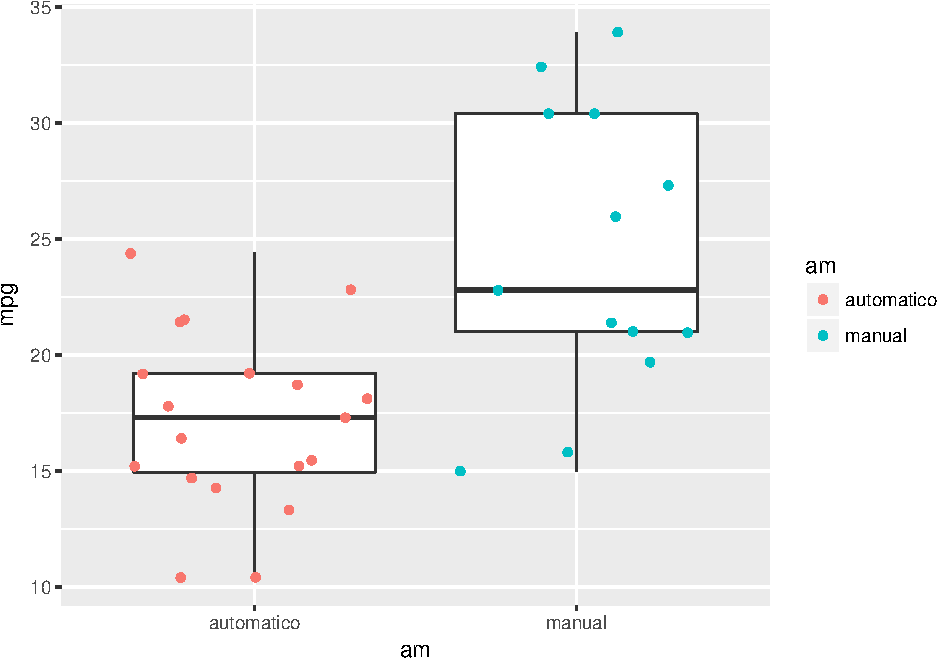
\includegraphics{Guia5_files/figure-latex/unnamed-chunk-2-1.pdf}
\caption{Comparación de eficiencia entre vehiculos automaticos y
manuales}
\end{figure}

Para hacer la comparación debemos agregar el argumento
\texttt{var.equal} el cual en este caso asumiremos que es verdad, ya que
en la próxima sección veremos los supuestos de la prueba t y las
consecuencias de las violaciones de estos supuestos. En este caso
podemos usar el simbolo \texttt{\textasciitilde{}} a ser leido como
explicado por para la prueba t de dos muestras.

\begin{Shaded}
\begin{Highlighting}[]
\KeywordTok{t.test}\NormalTok{(mpg }\OperatorTok{~}\StringTok{ }\NormalTok{am, }\DataTypeTok{data =}\NormalTok{ mtcars, }\DataTypeTok{var.equal =}\OtherTok{TRUE}\NormalTok{)}
\end{Highlighting}
\end{Shaded}

\begin{verbatim}
## 
##  Two Sample t-test
## 
## data:  mpg by am
## t = -4.1061, df = 30, p-value = 0.000285
## alternative hypothesis: true difference in means is not equal to 0
## 95 percent confidence interval:
##  -10.84837  -3.64151
## sample estimates:
## mean in group 0 mean in group 1 
##        17.14737        24.39231
\end{verbatim}

En este caso se determinaría que los vehiculos manuales (am = 1), son
más eficientes que sus contrapartes automáticas.

\paragraph{Ejercicio 2}\label{ejercicio-2}

Para el siguiente ejercicio usaremos la base de datos \texttt{BeerDark}
disponible en webcursos o en el siguiente
\href{https://archive.org/download/BeerDark/BeerDark.csv}{link}. Esta
base de datos posee 7 columnas, pero usaremos solo 4 de ellas:

\begin{itemize}
\tightlist
\item
  \textbf{Estilo:} Separa las cervezas entre Porters y Stouts
\item
  \textbf{Grado\_Alcoholico:} El grado alcoholico de las cervezas
\item
  \textbf{Amargor:} Valor IBU (International Bittering Units), a mayor
  valor más amarga la cerveza
\item
  \textbf{Color:} A mayor valor más oscura la cerveza.
\end{itemize}

Determinar si las cervezas Porter y Stouts son distintas en grado
alcoholico, amargor y/o color.

\subsection{Supuestos de la prueba de t y
alternativas}\label{supuestos-de-la-prueba-de-t-y-alternativas}

Los supuestos de la t de student son las siguientes (Boneau 1960)

\begin{itemize}
\tightlist
\item
  Independencia de las observaciones
\item
  Distribución normal de los datos en cada grupo
\item
  Homogeneidad de varianza
\end{itemize}

\subsubsection{Prueba de una muestra}\label{prueba-de-una-muestra}

Como siempre la independencia de las muestras es algo que solo puede
determinarse en base a el diseño del muestreo, y por otro lado, al haber
solo una muestra, la homogeneidad de varianza no es un problema, en este
caso solo podemos ver si la distribución es normal. Volviendo a nuestro
ejemplo de una muestra, con la base de datos \texttt{faithfull}, veamos
en base a un histograma (figura 2), qqplot (figura 3) y test de shapiro,
si los datos son normales o no:

\begin{Shaded}
\begin{Highlighting}[]
\KeywordTok{hist}\NormalTok{(faithful}\OperatorTok{$}\NormalTok{waiting, }\DataTypeTok{xlab =} \StringTok{"Minutos de espera entre erupciones"}\NormalTok{)}
\end{Highlighting}
\end{Shaded}

\begin{figure}
\centering
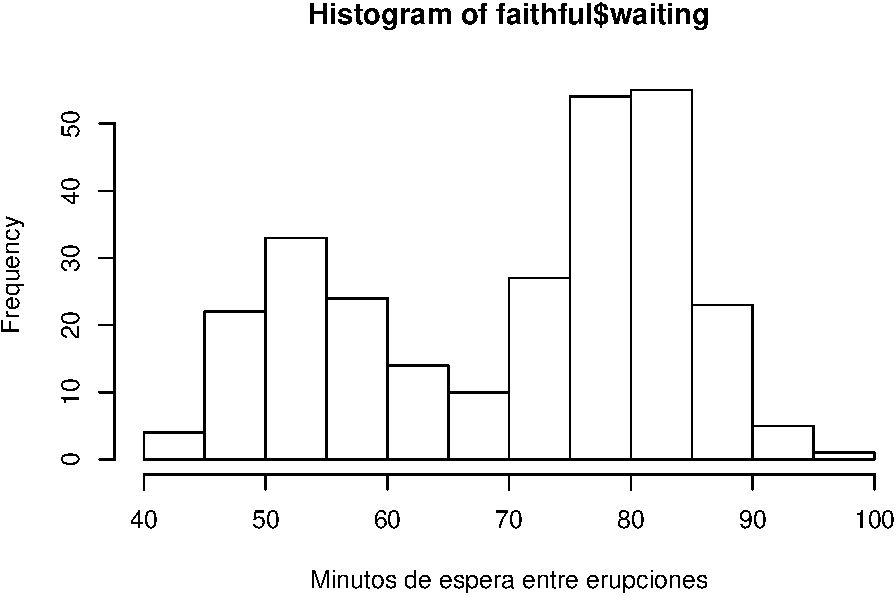
\includegraphics{Guia5_files/figure-latex/unnamed-chunk-4-1.pdf}
\caption{Histograma de los minutos de espera de el géiser Old Fiathful}
\end{figure}

\begin{Shaded}
\begin{Highlighting}[]
\KeywordTok{qqnorm}\NormalTok{(faithful}\OperatorTok{$}\NormalTok{waiting)}
\end{Highlighting}
\end{Shaded}

\begin{figure}
\centering
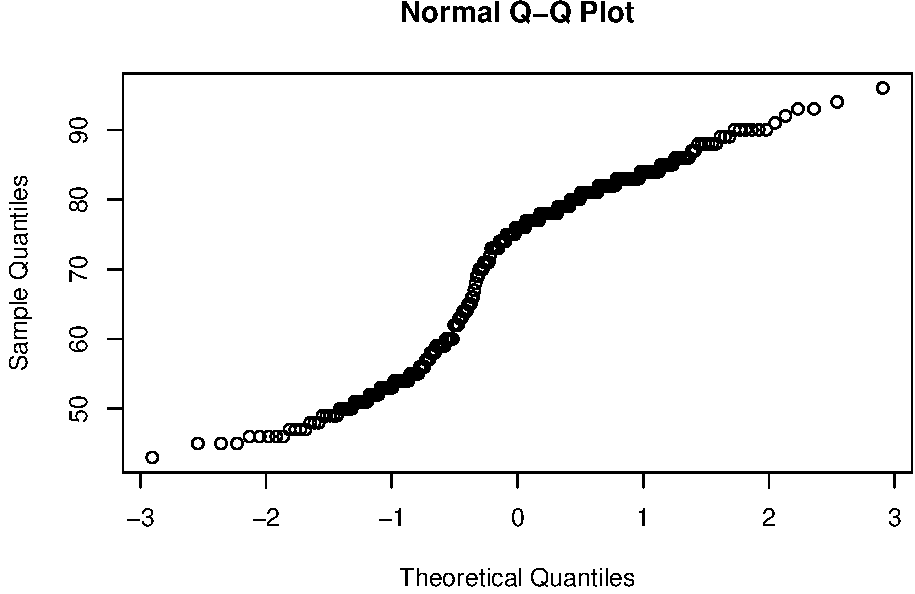
\includegraphics{Guia5_files/figure-latex/unnamed-chunk-5-1.pdf}
\caption{QQplot de los minutos de espera de el géiser Old Fiathful}
\end{figure}

\begin{Shaded}
\begin{Highlighting}[]
\KeywordTok{shapiro.test}\NormalTok{(faithful}\OperatorTok{$}\NormalTok{waiting)}
\end{Highlighting}
\end{Shaded}

\begin{verbatim}
## 
##  Shapiro-Wilk normality test
## 
## data:  faithful$waiting
## W = 0.92215, p-value = 1.015e-10
\end{verbatim}

Como vemos en la figura 2, los datos no se ven normales, incluso se ven
bimodales, lo cual significa que tiene 2 picos, en este caso uno al
rededor de los 52 minutos y otro al rededor de los 85 minutos de espera
(recordemos que la función \texttt{hist}, automáticamente usa el
algoritmo de Sturges (1926), para determinar como dividir los datos y
obtener el mejor histograma). Nuestras sospechas de no normalidad son
confirmadas al ver el qqplot, que no sigue para nada la diagonal, y es
reafirmado por el test de shapiro, cuyo valor mucho menor a 0.05, nos
dice que la distribución no es normal. Dado esto, debemos apelar a un
test de distribución libre como el de \emph{Mann-Whitney}, la cual se
realiza con la función \texttt{wilcox.test}, de la misma forma que es
utilizada la función \texttt{t.test}, por lo tanto para nuestro ejemplo
usamos:

\begin{Shaded}
\begin{Highlighting}[]
\KeywordTok{data}\NormalTok{(}\StringTok{"faithful"}\NormalTok{)}
\KeywordTok{wilcox.test}\NormalTok{(}\DataTypeTok{x =}\NormalTok{ faithful}\OperatorTok{$}\NormalTok{waiting, }\DataTypeTok{mu =} \DecValTok{60}\NormalTok{, }\DataTypeTok{alternative =} \StringTok{"two.sided"}\NormalTok{)}
\end{Highlighting}
\end{Shaded}

\begin{verbatim}
## 
##  Wilcoxon signed rank test with continuity correction
## 
## data:  faithful$waiting
## V = 31048, p-value < 2.2e-16
## alternative hypothesis: true location is not equal to 60
\end{verbatim}

Que en este caso nos lleva a la misma conclusión que nuestro ejemplo
anterior.

\subsubsection{Prueba de dos muestras}\label{prueba-de-dos-muestras}

Para una prueba de dos muestras, podemos testear tanto la homogeneidad
de varianza como la normalidad, para ver las dos cosas al mismo tiempo
podemos usar un gráfico de violín (figura 4). En este caso, las
distribuciones no se ven muy diferentes a la normalidad, pero las
varianzas se ven un tanto distintas, podemos seguir explorando esto
visualmente usando la función \texttt{hist} previamente generando dos
data frames, uno para autos automatico y otro para manuales.

\begin{Shaded}
\begin{Highlighting}[]
\KeywordTok{data}\NormalTok{(}\StringTok{"mtcars"}\NormalTok{)}
\NormalTok{mt <-}\StringTok{ }\NormalTok{mtcars}
\NormalTok{mt}\OperatorTok{$}\NormalTok{am <-}\StringTok{ }\KeywordTok{ifelse}\NormalTok{(mtcars}\OperatorTok{$}\NormalTok{am  }\OperatorTok{==}\StringTok{ }\DecValTok{0}\NormalTok{, }\StringTok{"automatico"}\NormalTok{, }\StringTok{"manual"}\NormalTok{)}
\NormalTok{mt <-}\StringTok{ }\KeywordTok{as.data.frame}\NormalTok{(mt)}
\KeywordTok{ggplot}\NormalTok{(mt, }\KeywordTok{aes}\NormalTok{(}\DataTypeTok{x =}\NormalTok{ am, }\DataTypeTok{y =}\NormalTok{ mpg)) }\OperatorTok{+}\StringTok{ }\KeywordTok{geom_violin}\NormalTok{()}
\end{Highlighting}
\end{Shaded}

\begin{figure}
\centering
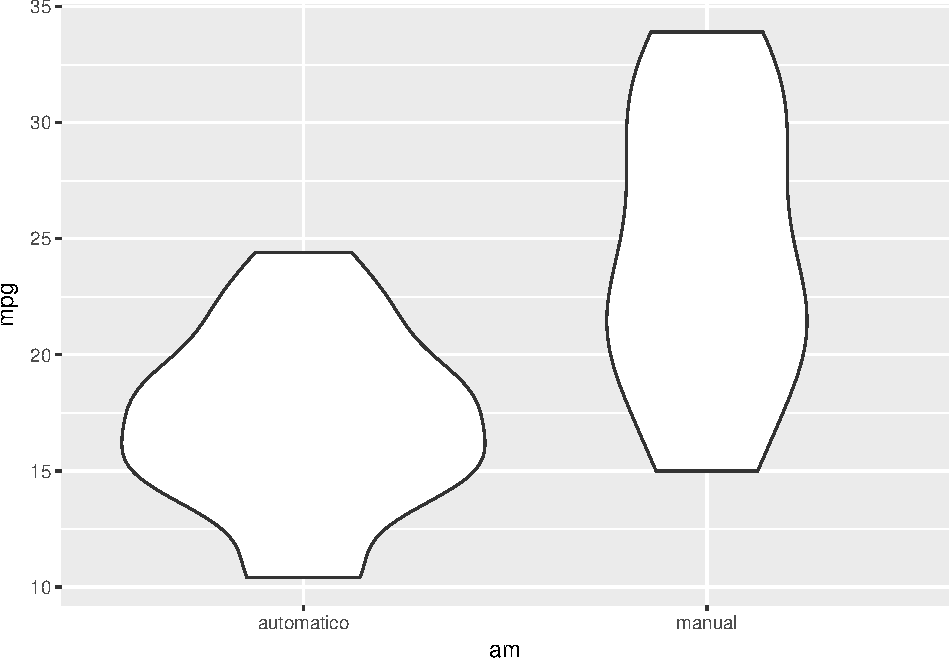
\includegraphics{Guia5_files/figure-latex/unnamed-chunk-8-1.pdf}
\caption{Comparación de distribuciones y varianzas de los vehiculos
automáticos}
\end{figure}

En este caso, las distribuciones no se ven muy diferentes a la
normalidad, pero las varianzas se ven un tanto distintas, podemos seguir
explorando esto separando los datos en vehiculos automáticos y manuales
para hacer histogramas, en este caso es importante que los ejes sean
iguales, para eso en el histograma usaremos los parametros ylim y xlim.

\begin{Shaded}
\begin{Highlighting}[]
\NormalTok{manuales <-}\StringTok{ }\NormalTok{mt }\OperatorTok\StringTok{ }\KeywordTok{filter}\NormalTok{(am }\OperatorTok{==}\StringTok{ "manual"}\NormalTok{)}
\KeywordTok{hist}\NormalTok{(manuales}\OperatorTok{$}\NormalTok{mpg, }\DataTypeTok{xlim =} \KeywordTok{c}\NormalTok{(}\DecValTok{10}\NormalTok{,}\DecValTok{35}\NormalTok{), }\DataTypeTok{ylim =} \KeywordTok{c}\NormalTok{(}\DecValTok{0}\NormalTok{,}\DecValTok{5}\NormalTok{))}
\end{Highlighting}
\end{Shaded}

\begin{figure}
\centering
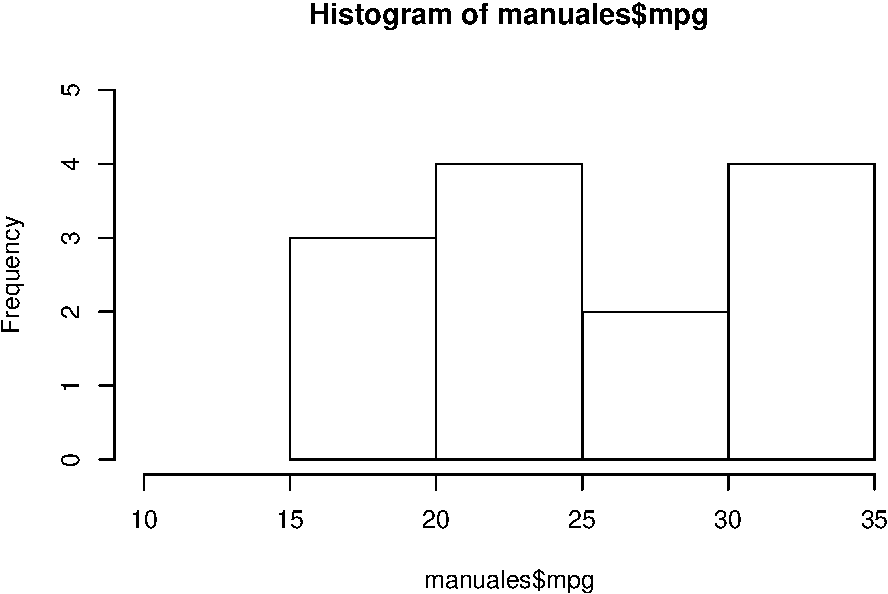
\includegraphics{Guia5_files/figure-latex/unnamed-chunk-9-1.pdf}
\caption{Histograma de vehiculos manuales}
\end{figure}

\begin{Shaded}
\begin{Highlighting}[]
\NormalTok{autos <-}\StringTok{ }\NormalTok{mt }\OperatorTok\StringTok{ }\KeywordTok{filter}\NormalTok{(am }\OperatorTok{==}\StringTok{ "automatico"}\NormalTok{)}
\KeywordTok{hist}\NormalTok{(autos}\OperatorTok{$}\NormalTok{mpg, }\DataTypeTok{xlim =} \KeywordTok{c}\NormalTok{(}\DecValTok{10}\NormalTok{,}\DecValTok{35}\NormalTok{), }\DataTypeTok{ylim =} \KeywordTok{c}\NormalTok{(}\DecValTok{0}\NormalTok{,}\DecValTok{5}\NormalTok{))}
\end{Highlighting}
\end{Shaded}

\begin{figure}
\centering
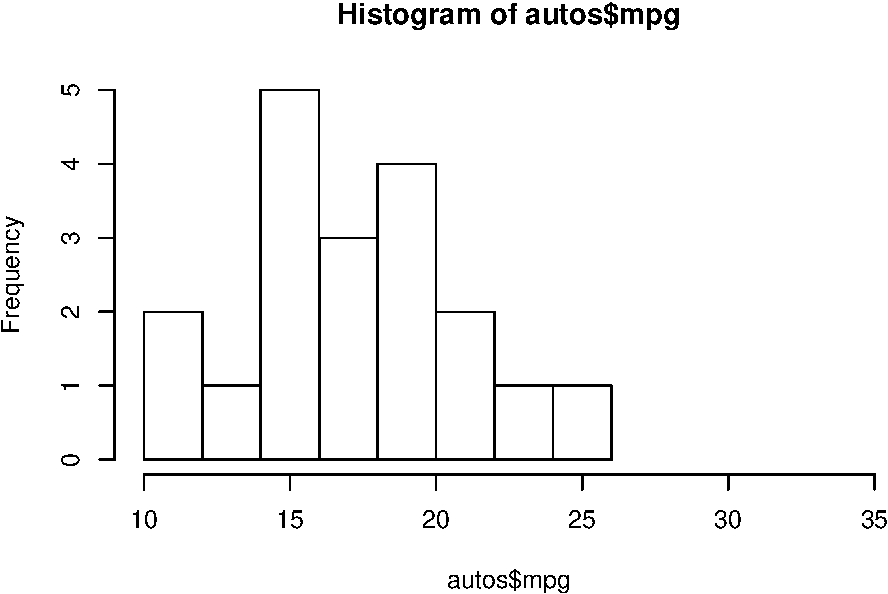
\includegraphics{Guia5_files/figure-latex/unnamed-chunk-10-1.pdf}
\caption{Histograma de vehiculos automáticos}
\end{figure}

Como vemos, los vehículos manuales no parecen tener distribución normal
como se ve en la figura 5, esto podemos comprobarlo con el qqlot de los
mismos datos (figura 5)

\begin{Shaded}
\begin{Highlighting}[]
\KeywordTok{qqnorm}\NormalTok{(manuales}\OperatorTok{$}\NormalTok{mpg)}
\end{Highlighting}
\end{Shaded}

\begin{figure}
\centering
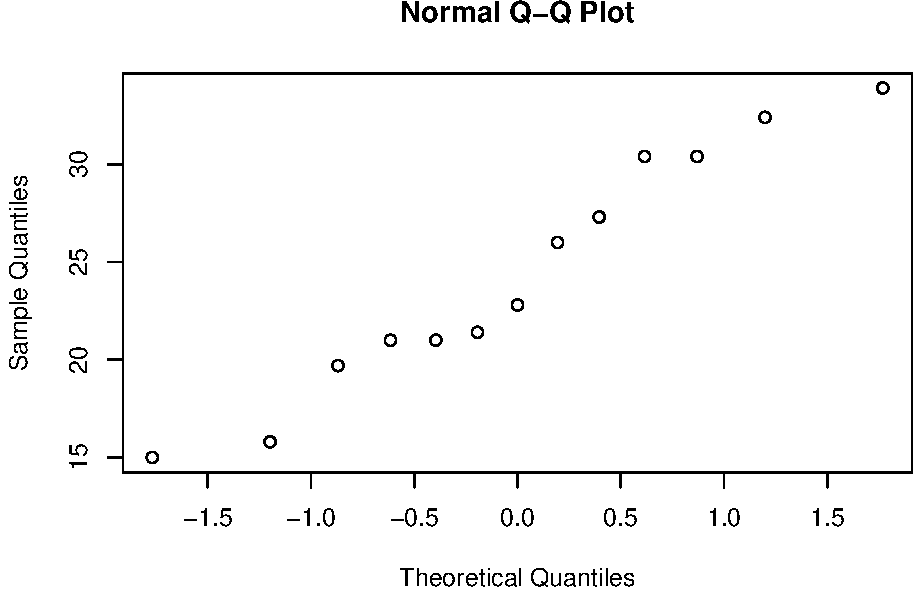
\includegraphics{Guia5_files/figure-latex/unnamed-chunk-11-1.pdf}
\caption{QQplot de eficiencia de vehiculos con cambios manuales}
\end{figure}

\paragraph{Ejercicio 3}\label{ejercicio-3}

Como siempre la independencia de las muestras es algo que solo puede
determinarse en base a el diseño del muestreo, y por otro lado, al haber
solo una muestra, la homogeneidad de varianza no es un problema, en este
caso solo podemos ver si la distribución es normal. Volviendo a nuestro
ejercicio de una muestra, con la base de datos \texttt{airquality},
evalue basado en histograma, qqplot y test de shapiro si se debe
reevaluar la hipótesis para los meses de julio y agosto

Para una prueba de dos muestras, podemos testear tanto la homogeneidad
de varianza como la normalidad, para ver las dos cosas al mismo tiempo
podemos usar un gráfico de violín \texttt{geom\_violin} en
\emph{ggplot2}, lo cual puede seguir siendo explorando esto visualmente
usando la función \texttt{hist} generando dos data frames, uno por cada
clase de datos.

Evalúe si es necesario revaluar la hipotesis de que el amargor es
distinto entre ambos estilos de cerveza

\subsection*{Bibliografía}\label{bibliografia}
\addcontentsline{toc}{subsection}{Bibliografía}

\hypertarget{refs}{}
\hypertarget{ref-azzalini1990look}{}
Azzalini, Adelchi, and Adrian W Bowman. 1990. ``A Look at Some Data on
the Old Faithful Geyser.'' \emph{Applied Statistics}. JSTOR, 357--65.

\hypertarget{ref-boneau1960effects}{}
Boneau, C Alan. 1960. ``The Effects of Violations of Assumptions
Underlying the T Test.'' \emph{Psychological Bulletin} 57 (1). American
Psychological Association: 49.

\hypertarget{ref-chambers35graphical}{}
Chambers, John M, William S Cleveland, Beat Kleiner, and Paul A Tukey.
1983. ``Graphical Methods for Data Analysis. 1983.'' \emph{Wadsworth,
Belmont, CA} 35.

\hypertarget{ref-student1908probable}{}
Student. 1908. ``The Probable Error of a Mean.'' \emph{Biometrika}.
JSTOR, 1--25.

\hypertarget{ref-sturges1926choice}{}
Sturges, Herbert A. 1926. ``The Choice of a Class Interval.''
\emph{Journal of the American Statistical Association} 21 (153): 65--66.


\end{document}
